\begin{center}

\includegraphics[width=0.5\textwidth]{content/3/chapter7/images/18.png}\\
Cippi digs the garden
\end{center}

Before I modify the workflow from section co\_await, I want to make the awaiter workflow more transparent.


\subsubsubsection{7.4.1\hspace{0.2cm} The Transparent Awaiter Workflow}

I added a few output messages to the program startJob.cpp.

\hspace*{\fill} \\ %插入空行
\noindent
Starting a job on request (including comments)
\begin{lstlisting}[style=styleCXX]
// startJobWithComments.cpp

#include <coroutine>
#include <iostream>

struct MySuspendAlways {
	bool await_ready() const noexcept {
		std::cout << " MySuspendAlways::await_ready" << '\n';
		return false;
	}
	void await_suspend(std::coroutine_handle<>) const noexcept {
		std::cout << " MySuspendAlways::await_suspend" << '\n';
	
	}
	void await_resume() const noexcept {
		std::cout << " MySuspendAlways::await_resume" << '\n';
	}
};

struct MySuspendNever {
	bool await_ready() const noexcept {
		std::cout << " MySuspendNever::await_ready" << '\n';
		return true;
	}
	void await_suspend(std::coroutine_handle<>) const noexcept {
		std::cout << " MySuspendNever::await_suspend" << '\n';
	
	}
	void await_resume() const noexcept {
		std::cout << " MySuspendNever::await_resume" << '\n';
	}
};
	
struct Job {
	struct promise_type;
	using handle_type = std::coroutine_handle<promise_type>;
	handle_type coro;
	Job(handle_type h): coro(h){}
	~Job() {
		if ( coro ) coro.destroy();
	}
	void start() {
		coro.resume();
	}
	
	
	struct promise_type {
		auto get_return_object() {
			return Job{handle_type::from_promise(*this)};
		}
		MySuspendAlways initial_suspend() {
			std::cout << " Job prepared" << '\n';
			return {};
		}
		MySuspendAlways final_suspend() noexcept {
			std::cout << " Job finished" << '\n';
			return {};
		}
		void return_void() {}
		void unhandled_exception() {}
	
	};
};

Job prepareJob() {
	co_await MySuspendNever();
}

int main() {

	std::cout << "Before job" << '\n';
	
	auto job = prepareJob();
	job.start();
	
	std::cout << "After job" << '\n';

}
\end{lstlisting}

First of all, I replaced the predefined Awaitables std::suspend\_always and std::suspend\_never with Awaitables MySuspendAlways (line 6) and MySuspendNever (line 20). I use them in lines 51, 55, and 66. The Awaitables mimic the behavior of the predefined Awaitables but additionally write a comment. Due to the use of std::cout, the member functions await\_ready, await\_suspend, and await\_resume cannot be declared as constexpr.

The screenshot of the program execution shows the control flow nicely, which you can directly observe on the \href{https://godbolt.org/z/T5rcE4}{Compiler Explorer}.

\begin{center}
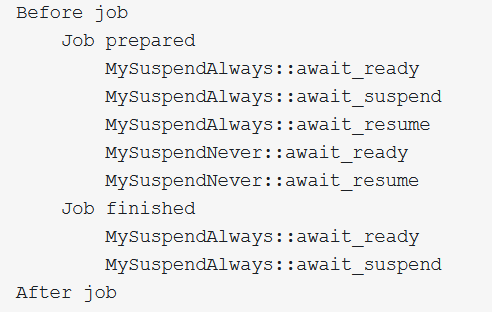
\includegraphics[width=0.8\textwidth]{content/3/chapter7/images/19.png}\\
Starting a job on request (including comments)
\end{center}

The function initial\_suspend (line 51) is executed at the beginning of the coroutine and the function final\_suspend at its end (line 55). The call prepareJob() (line 73) triggers the creation of the coroutine object, and the function call job.start() its resumption and, hence, completion (line 74). Consequently, the members await\_ready, await\_suspend, and await\_resume of MySuspendAlways are executed. When you don’t resume the Awaitable such as the coroutine object returned by the member function final\_suspend, the function await\_resume is not processed. In contrast, the Awaitable’s MySuspendNever function is immediately ready because await\_ready returns true and, hence, does not suspend. Thanks to the comments, you should have an elementary understanding of the awaiter workflow.

Now, it’s time to vary it.

\subsubsubsection{7.4.2\hspace{0.2cm} Automatically Resuming the Awaiter}

In the previous workflow, I explicitly started the job.

\hspace*{\fill} \\ %插入空行
\noindent
Explicitly starting the job
\begin{lstlisting}[style=styleCXX]
int main() {
	
	std::cout << "Before job" << '\n';
	
	auto job = prepareJob();
	job.start();
	
	std::cout << "After job" << '\n';
	
}
\end{lstlisting}

This explicit invoking of job.start() was necessary because await\_ready in the Awaitable MySuspendAlways always returned false. Now let’s assume that await\_ready can return true or false and the job is not explicitly started. A short reminder: When await\_ready returns true, the function await\_resume is directly invoked but not await\_suspend.

\hspace*{\fill} \\ %插入空行
\noindent
Automatically Resuming the Awaiter
\begin{lstlisting}[style=styleCXX]
// startJobWithAutomaticResumption.cpp

#include <coroutine>
#include <functional>
#include <iostream>
#include <random>

std::random_device seed;
auto gen = std::bind_front(std::uniform_int_distribution<>(0,1),
						   std::default_random_engine(seed()));

struct MySuspendAlways {
	bool await_ready() const noexcept {
		std::cout << " MySuspendAlways::await_ready" << '\n';
		return gen();
	}
	bool await_suspend(std::coroutine_handle<> handle) const noexcept {
		std::cout << " MySuspendAlways::await_suspend" << '\n';
		handle.resume();
		return true;
	
	}
	void await_resume() const noexcept {
		std::cout << " MySuspendAlways::await_resume" << '\n';
	}
};

struct Job {
	struct promise_type;
	using handle_type = std::coroutine_handle<promise_type>;
	handle_type coro;
	Job(handle_type h): coro(h){}
	~Job() {
		if ( coro ) coro.destroy();
	}
	
	struct promise_type {
		auto get_return_object() {
			return Job{handle_type::from_promise(*this)};
		}
		MySuspendAlways initial_suspend() {
		std::cout << " Job prepared" << '\n';
			return {};
		}
		std::suspend_always final_suspend() noexcept {
			std::cout << " Job finished" << '\n';
			return {};
		}
		void return_void() {}
		void unhandled_exception() {}
	
	};
};

Job performJob() {
	co_await std::suspend_never();
}

int main() {

	std::cout << "Before jobs" << '\n';
	
	performJob();
	performJob();
	performJob();
	performJob();
	
	std::cout << "After jobs" << '\n';

}
\end{lstlisting}

irst of all, the coroutine is now called performJob and runs automatically. gen (line 9) is a random number generator for the numbers 0 or 1. It uses for its job the default random engine, initialized with the seed. Thanks to std::bind\_front, I can bind it together with the std::uniform\_int\_distribution to get a callable which, when used, gives me a random number 0 or 1.

I removed in this example the Awaitables with predefined Awaitables from the C++ standard, except the Awaitable MySuspendAlways as the return type of the member function initial\_suspend (line 41). await\_ready (line 13) returns a boolean. When the boolean is true, the control flow jumps directly to the member function await\_resume (line 23), when false, the coroutine is immediately suspended and, therefore, the function await\_suspend runs (line 17). The function await\_suspend gets the handle to the coroutine and uses it to resume the coroutine (line 19). Instead of returning the value true, await\_suspend can also return void.

The following screenshot shows: When await\_ready returns true, the function await\_resume is called, when await\_ready returns false, the function await\_suspend is also called.

You can try out the program on the \href{https://godbolt.org/z/8b1Y14}{Compiler Explorer}.

\begin{center}
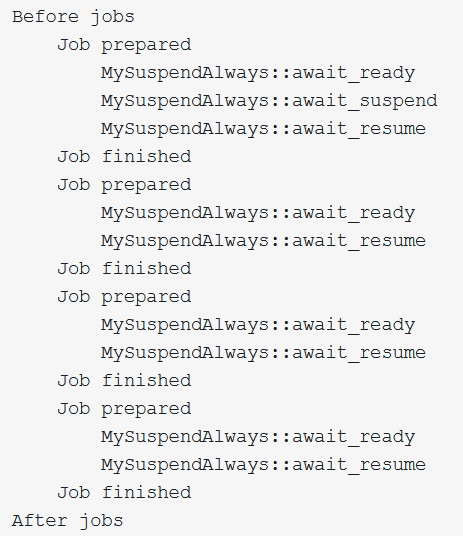
\includegraphics[width=0.8\textwidth]{content/3/chapter7/images/20.png}\\
Automatically Resuming the Awaiter
\end{center}

Let me improve the presented program more and resume the awaiter on a separate thread.

\subsubsubsection{7.4.3\hspace{0.2cm} Automatically Resuming the Awaiter on a Separate Thread}

The following program is based on the previous one.

\hspace*{\fill} \\ %插入空行
\noindent
Automatically Resuming the Awaiter on a Seperate Thread
\begin{lstlisting}[style=styleCXX]
// startJobWithAutomaticResumptionOnThread.cpp

#include <coroutine>
#include <functional>
#include <iostream>
#include <random>
#include <thread>
#include <vector>

std::random_device seed;
auto gen = std::bind_front(std::uniform_int_distribution<>(0,1),
						   std::default_random_engine(seed()));

struct MyAwaitable {
	std::jthread& outerThread;
	bool await_ready() const noexcept {
		auto res = gen();
		if (res) std::cout << " (executed)" << '\n';
		else std::cout << " (suspended)" << '\n';
		return res;
	}
	void await_suspend(std::coroutine_handle<> h) {
		outerThread = std::jthread([h] { h.resume(); });
	}
	void await_resume() {}
};


struct Job{
	static inline int JobCounter{1};
	Job() {
		++JobCounter;
	}

	struct promise_type {
		int JobNumber{JobCounter};
		Job get_return_object() { return {}; }
		std::suspend_never initial_suspend() {
			std::cout << " Job " << JobNumber << " prepared on thread "
			          << std::this_thread::get_id();
			return {};
		}
		std::suspend_never final_suspend() noexcept {
			std::cout << " Job " << JobNumber << " finished on thread "
			          << std::this_thread::get_id() << '\n';
			return {};
		}
		void return_void() {}
		void unhandled_exception() { }
	};
};

Job performJob(std::jthread& out) {
	co_await MyAwaitable{out};
}

int main() {

	std::vector<std::jthread> threads(8);
	for (auto& thr: threads) performJob(thr);

}
\end{lstlisting}

The main difference with the previous program is the new awaitable MyAwaitable, used in the coroutine performJob (line 54). On the contrary, the coroutine object returned from the coroutine performJob is straightforward. Essentially, its member functions initial\_suspend (line 38) and final\_suspend (line 43) return the predefined awaitable std::suspend\_never. Additionally, both functions show the JobNumber of the executed job and the thread ID on which it runs. The screenshot shows which coroutine runs immediately and which one is suspended. Thanks to the thread id, you can observe that suspended coroutines are resumed on a different thread.

You can try out the program on the \href{https://wandbox.org/permlink/skHgWKF0SYAwp8Dm}{Wandbox}.

\begin{center}
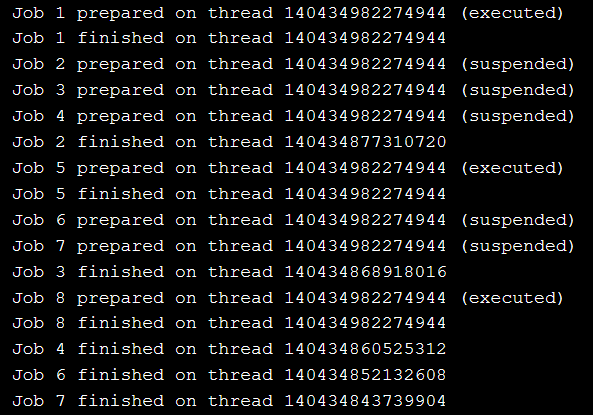
\includegraphics[width=0.8\textwidth]{content/3/chapter7/images/21.png}\\
Automatically Resuming the Awaiter on a Separate Thread
\end{center}

Let me discuss the interesting control flow of the program. Line 59 creates eight default-constructed threads, which the coroutine performJob (line 53) takes by reference. Further, the reference becomes the argument for creating MyAwaitable\{out\} (line 54). Depending on the value of res (line 17), and, therefore, the return value of the function await\_ready, the Awaitable continues (res is true) to run or is suspended (res is false). In case MyAwaitable is suspended, the function await\_suspend (line 22) is executed. Thanks to the assignment of outerThread (line 23), it becomes a running thread. The running threads must outlive the lifetime of the coroutine. For this reason, the threads have the scope of the main function.

\begin{tcolorbox}[breakable,enhanced jigsaw,colback=mygreen!5!white,colframe=mygreen!75!black,title={Distilled Information}]
	
\begin{itemize}
\item 
When you want to synchronize threads more than once, you have many options. You can use condition variables, std::atomic\_flag, std::atomic<bool>, or semaphores. This case study answers the question: Which variant is the fastest one? The numbers show that condition variables are the slowest way, and atomic flags the fastest way to synchronize threads. The performance of std::atomic<bool> is in between. Semaphores are nearly as fast as atomic flags.

\item 
The section coroutines introduced an eager future, using co\_return. This future is an ideal starting point to make it lazy and finally, let it run on its own thread.

\item 
Modifications of the generator for an infinite data stream reveals its nature. When the member function initial\_suspend returns std::suspend\_never, the coroutine starts immediately and ignores the first value. In contrast, returning std::suspend\_never from the function yield\_value ends in an infinite loop. When you forget to resume the coroutine, it will never run.

\item 
The generator Generator<T> is generally applicable. Instead of an infinite data stream, it can successively return the elements of an arbitrary container of the Standard Template Library.

\item 
Implementing your own Awaitable MySuspendNever and MySuspendAlways makes the awaiter workflow transparent. Adapting the Awaitable MySuspendAlways enables it to create an Awaiter that resumes itself if necessary.

\item 
Modification of the Awaitable empowers you to automatically resume the coroutine on a separate thread.
\end{itemize}
	
\end{tcolorbox}




















